\documentclass[preprint,11pt]{elsarticle}

\usepackage{amsmath,amssymb}
\usepackage{graphicx}
\usepackage{booktabs}
\usepackage{algorithm}
\usepackage{algpseudocode}
\usepackage[hidelinks]{hyperref}
\usepackage[capitalise,noabbrev]{cleveref}
\usepackage{xcolor}
\usepackage[margin=2.5cm]{geometry}

\graphicspath{{../results/figures/}}
\newcommand{\R}{\mathbb{R}}
\newcommand{\norm}[1]{\lVert #1\rVert}
\DeclareMathOperator*{\argmin}{arg\,min}

\journal{Course Project Report, Prince Sattam bin Abdulaziz University}

\begin{document}

\begin{frontmatter}

\title{ASH-LR: Adaptive and Numerically Stable Optimization for Ill-Conditioned Logistic Regression}

\author{Saad Almusfir}
\ead{info@saad-group.net}
\affiliation{organization={College of Computer Engineering and Science, Prince Sattam bin Abdulaziz University},
            city={Al-Kharj},
            country={Saudi Arabia}}

\begin{abstract}
Fitting $\ell_2$-regularized logistic regression is slow for first-order methods when
features are correlated or differently scaled, and naive evaluation of the loss can
overflow. We study Adaptive Stable Hybrid Logistic Regression (ASH-LR), which combines
overflow-free evaluation of the loss, an initial phase of gradient steps, and a damped
inexact Newton phase in which $(H+\mu I)p=-g$ is solved by conjugate gradients using
Hessian-vector products, with $\mu=\sqrt{\theta\lVert g\rVert}$ and $\theta$ adapted by
a ratio test. Following a pre-registered plan, we compare ASH-LR with gradient descent,
Newton's method, Newton--CG and L-BFGS on eight regimes (synthetic designs with
condition numbers up to $10^{6}$, badly scaled features, and the Spambase data set),
ten seeds each, and complement the comparison with robustness, ablation,
single-precision and stability experiments. ASH-LR converged on all problems, whereas
L-BFGS failed on the larger and badly scaled ones, and stable evaluation was essential
from distant starting points. The pre-registered hypothesis of a 20\% reduction in
work relative to the best matrix-free baseline was not supported: ASH-LR needed
18--127\% more data passes than Newton--CG in four of five ill-conditioned regimes and
was statistically on a par in the fifth, and direct Newton was fastest for all dimensions studied
($d\le500$). The ablation attributes the gap to the gradient phase and, on badly scaled
data, to the accuracy of the unpreconditioned inner solver rather than to damping.
\end{abstract}

\begin{keyword}
logistic regression \sep ill-conditioning \sep inexact Newton method \sep conjugate gradient \sep regularized Newton \sep numerical stability
\end{keyword}

\end{frontmatter}

\section{Introduction}\label{sec:intro}

Logistic regression remains one of the most widely used models for binary
classification, and fitting it is a smooth, strongly convex optimization problem
when an $\ell_2$ penalty is added. In practice the problem is often
\emph{ill-conditioned}: features are strongly correlated, measured on very different
scales, or both, so that the Hessian of the objective has eigenvalues spread over
many orders of magnitude. First-order methods then converge slowly, because their
step size is limited by the largest curvature while progress along low-curvature
directions is proportional to the smallest one~\cite{wright2022optimization,berahas2020investigation}.
Newton-type methods are insensitive to this spread in theory, but they require
second-order information, can take poor steps far from the solution, and, in their
textbook form, solve a dense linear system whose cost grows as $O(nd^2+d^3)$.

A second, more mundane difficulty is numerical. Evaluating
$\log(1+e^{-z})$ and the sigmoid $1/(1+e^{-z})$ directly overflows once $|z|$
exceeds roughly $709$ in double precision and $88$ in single precision. Such
margins arise when features are unscaled, when the starting point is far from the
solution, or when the data are nearly separable, and an overflowing loss silently
breaks line searches and acceptance tests~\cite{blanchard2021accurately,wiemann2024softplus}.

This report studies \emph{Adaptive Stable Hybrid Logistic Regression} (ASH-LR), a
method that combines (i) overflow-free evaluation of the loss and its derivatives,
(ii) an initial phase of inexpensive gradient steps followed by a one-way switch to
second-order steps, and (iii) a damped inexact Newton phase in which the system
$(H+\mu I)p=-g$ is solved by conjugate gradients (CG) using Hessian-vector
products only, and the damping $\mu$ is adapted by a ratio test that compares the
actual with the predicted decrease. In the final version the damping follows the
gradient-regularized rule $\mu_k=\sqrt{\theta_k\norm{g_k}}$, which is motivated by
recent regularized Newton methods~\cite{mishchenko2023regularized,doikov2024super}
and vanishes automatically near the solution.

The project went through two stages. A preliminary version (Milestone~2) used
direct linear solves and line-search-based damping; it converged on all test
problems but needed more iterations and more time than plain Newton. Exploratory
runs then showed that the halving damping rule kept steps over-damped for many
iterations. The final method replaces it, and the final evaluation was fixed in a
pre-registered plan, committed to the code repository before the final experiments
were run, to avoid selecting favourable test cases after the fact.

\paragraph{Research question} Can combining gradient steps with a damped,
matrix-free Newton--CG phase improve the robustness and the work-to-accuracy of
ill-conditioned logistic regression, compared with established matrix-free
methods (Newton--CG and L-BFGS)? The pre-registered success criterion (H1) is a
reduction of at least $20\%$ in the median number of data passes relative to the
best converging matrix-free baseline in at least two of five predeclared
ill-conditioned regimes.

\paragraph{Contributions}
\begin{itemize}
  \item A complete, documented and tested implementation of ASH-LR and five
  baselines with a common interface, an exact work counter in units of data passes,
  and a generator of synthetic designs with an exactly prescribed condition number.
  \item A pre-registered evaluation on eight regimes (six synthetic, two based on the
  Spambase data set) with ten seeds each, complemented by robustness, ablation,
  single-precision and stability experiments.
  \item An honest assessment: we report where ASH-LR helps, where it does not, and
  why direct Newton remains the method of choice for small dense problems.
\end{itemize}

The rest of the report is organized as follows. \Cref{sec:related} reviews related
work, \cref{sec:method} formulates the problem and the algorithm,
\cref{sec:setup} describes the experimental setup, \cref{sec:results} presents and
discusses the results, and \cref{sec:conclusion} concludes.

\section{Related work}\label{sec:related}

\paragraph{Optimizers for logistic regression}
Minka~\cite{minka2003comparison} compared gradient, conjugate-gradient, quasi-Newton
and Newton (iteratively reweighted least squares) methods for logistic regression
and found Newton-type methods fastest for small and medium dimension, with the cost
of the dense Hessian becoming limiting as $d$ grows. Lin, Weng and
Keerthi~\cite{lin2008trust} proposed a trust-region Newton method in which each
subproblem is solved by CG with Hessian-vector products; it became the default
large-scale solver in LIBLINEAR and is the closest relative of the second phase of
ASH-LR. Limited-memory BFGS~\cite{liu1989limited} is the other standard
matrix-free choice and serves as a baseline here. Bach~\cite{bach2010self} showed
that the logistic loss is generalized self-concordant, which explains why Newton's
method behaves well for this problem in practice.

\paragraph{Inexact Newton methods}
Dembo, Eisenstat and Steihaug~\cite{dembo1982inexact} established that Newton's
method retains local linear, superlinear or quadratic convergence when the linear
system is solved only to a relative residual $\eta_k$ (the \emph{forcing term}),
provided $\eta_k$ is bounded away from one, tends to zero, or tends to zero as
$O(\norm{g_k})$, respectively. Eisenstat and Walker~\cite{eisenstat1996forcing}
studied adaptive choices of $\eta_k$. We use the classical choice
$\eta_k=\min(0.5,\sqrt{\norm{g_k}})$, which yields superlinear local
convergence~\cite[Thm.~7.2]{nocedal2006numerical}. Conjugate
gradients~\cite{hestenes1952methods} are the natural inner solver because the
damped Hessian is symmetric positive definite. Hessian-free methods of this type
are also used in machine learning more broadly~\cite{martens2010deep,byrd2011stochastic}.

\paragraph{Damping and regularized Newton methods}
Adding $\mu I$ to the Hessian dates back to Levenberg~\cite{levenberg1944method} and
Marquardt~\cite{marquardt1963algorithm}; adapting $\mu$ by comparing actual and
predicted decrease is the standard trust-region mechanism~\cite{nocedal2006numerical}.
Li, Fukushima, Qi and Yamashita~\cite{li2004regularized} analysed regularized
Newton methods for convex problems with $\mu_k$ proportional to a power of
$\norm{g_k}$ and showed fast local convergence even with singular Hessians.
Mishchenko~\cite{mishchenko2023regularized} proved that the simple choice
$\mu_k=\sqrt{H\norm{g_k}}$, with $H$ the Lipschitz constant of the Hessian, gives a
global $O(1/k^2)$ rate together with local superlinear convergence, without line
search, matching cubic regularization~\cite{nesterov2006cubic} at the cost of one
linear solve per iteration. Doikov, Mishchenko and
Nesterov~\cite{doikov2024super} extended this to a \emph{super-universal} method
that adapts the regularization constant and the power of the gradient norm
automatically and evaluated it on logistic regression. ASH-LR borrows the
form $\mu_k=\sqrt{\theta_k\norm{g_k}}$ from this line of work and adapts
$\theta_k$ with a ratio test; the theoretical guarantees of
\cite{mishchenko2023regularized,doikov2024super} rely on their exact update rules
and on exact linear solves, and therefore do not transfer directly to ASH-LR.

\paragraph{Numerical stability}
Evaluating the softplus function $\log(1+e^{t})$ stably is a well-known
issue~\cite{higham2002accuracy}; Wiemann, Kneib and
Hambuckers~\cite{wiemann2024softplus} discuss the softplus identity in the context
of link functions for generalized linear models. We use the equivalent
\texttt{logaddexp} formulation and a sign-dependent sigmoid.

\paragraph{Adaptive second-order methods for streaming data}
Godichon-Baggioni and Werge~\cite{godichon2025adaptive} develop inversion-free
stochastic Newton methods with $O(dN)$ cost for ill-conditioned streaming problems,
illustrating both the benefit and the expense of curvature information. Our setting
is deterministic batch optimization, but the trade-off between the cost of curvature
information and the iterations it saves is the same question we study.

\section{Problem formulation and method}\label{sec:method}

\subsection{Objective}
Given observations $(x_i,y_i)$, $i=1,\dots,n$, with $x_i\in\R^d$ and
$y_i\in\{-1,+1\}$, we minimize
\begin{equation}\label{eq:obj}
  F(w)=\frac1n\sum_{i=1}^n \log\bigl(1+e^{-z_i}\bigr)+\frac\lambda2\norm{w}_2^2,
  \qquad z_i=y_i\,x_i^\top w,
\end{equation}
with $\lambda=10^{-6}$ unless stated otherwise and no separate intercept. Writing
$X\in\R^{n\times d}$ for the design matrix and $\sigma(t)=1/(1+e^{-t})$,
\begin{equation}\label{eq:derivs}
  \nabla F(w)=-\frac1n X^\top\bigl(y\odot\sigma(-z)\bigr)+\lambda w,\qquad
  \nabla^2F(w)=\frac1n X^\top D X+\lambda I,\quad D=\operatorname{diag}\bigl(\sigma(z_i)(1-\sigma(z_i))\bigr).
\end{equation}
Since $\lambda>0$, $F$ is $\lambda$-strongly convex and has a unique minimizer $w^*$.
The weights $D_{ii}\le 1/4$ vanish for large $|z_i|$, so the Hessian inherits and
can amplify the ill-conditioning of $X^\top X/n$: its smallest eigenvalue can be as
small as $\lambda$.

\subsection{Stable evaluation}
The loss term is evaluated as $\log(1+e^{-z})=\texttt{logaddexp}(0,-z)$, which
computes $\max(0,-z)+\log(1+e^{-|z|})$ and never exponentiates a positive number.
The sigmoid uses $\sigma(t)=1/(1+e^{-t})$ for $t\ge0$ and $e^{t}/(1+e^{t})$ for
$t<0$. Both forms are exact reformulations, so they change nothing when the naive
formulas do not overflow. For the ablation in \cref{sec:results} we also implement the
naive formulas $\log(1+e^{-z})$ and $1/(1+e^{-z})$.

\subsection{Search directions and line search}
Let $g_k=\nabla F(w_k)$ and $H_k=\nabla^2F(w_k)$. The methods compared use
\begin{align*}
  \text{GD:}&\quad p_k=-g_k, &
  \text{Newton:}&\quad H_kp_k=-g_k \ \text{(dense solve)},\\
  \text{Newton--CG:}&\quad H_kp_k\approx-g_k \ \text{(CG)}, &
  \text{ASH-LR (phase 2):}&\quad (H_k+\mu_kI)p_k\approx-g_k \ \text{(CG)}.
\end{align*}
L-BFGS uses the two-loop recursion with memory $m=10$ and skips curvature pairs
with $s^\top y\le10^{-10}\norm{s}\norm{y}$. Except for GD with fixed step $1/L$,
$L=\norm{X}_2^2/(4n)+\lambda$, all line searches use Armijo
backtracking~\cite{armijo1966minimization}: starting from $\alpha=1$, the step is
halved until $F(w_k+\alpha p_k)\le F(w_k)+c\,\alpha\, g_k^\top p_k$ with $c=10^{-4}$,
for at most 40 trials.

\subsection{Inexact solves with Hessian-vector products}
The product $(H_k+\mu I)v=\frac1n X^\top\bigl(D_k(Xv)\bigr)+(\lambda+\mu)v$
costs two passes over the data and never forms $H_k$. CG is run on
$(H_k+\mu_kI)p=-g_k$ from $p=0$ and stopped when the residual
$r=-g_k-(H_k+\mu_kI)p$ satisfies
\begin{equation}\label{eq:forcing}
  \norm{r}\le\eta_k\norm{g_k},\qquad \eta_k=\min\bigl(0.5,\sqrt{\norm{g_k}}\bigr),
\end{equation}
or after $d$ iterations. Because $H_k+\mu_kI$ is positive definite, every CG
iterate is a descent direction~\cite{nocedal2006numerical}.

\subsection{Switching rule}
ASH-LR starts with Armijo gradient steps and switches, once and for all, to the
damped Newton phase as soon as either
(i) $\norm{g_k}\le 0.1\,\norm{g_0}$, or
(ii) at least five gradient steps have been taken and the last step achieved a relative
decrease $(F(w_{k-1})-F(w_k))/\max(1,|F(w_k)|)\le10^{-3}$.
The idea is that cheap gradient steps make fast progress while far from the solution
and while the curvature model is unreliable, and that Newton steps take over when
gradient steps stall on the low-curvature directions.

\subsection{Damping by a ratio test}
For a trial direction $p$ the quadratic model predicts the decrease
\begin{equation}\label{eq:pred}
  \mathrm{pred}(p)=-\bigl(g_k^\top p+\tfrac12 p^\top H_kp\bigr).
\end{equation}
With an inexact solve, $(H_k+\mu_kI)p=-g_k-r$, so
$p^\top H_kp=-p^\top g_k-p^\top r-\mu_k\norm{p}^2$ is available from CG quantities
without an extra Hessian-vector product. The ratio
$\rho=\bigl(F(w_k)-F(w_k+p)\bigr)/\mathrm{pred}(p)$ measures how well the model
predicted the actual decrease. The step is accepted with $\alpha=1$ if
$\rho\ge10^{-4}$; otherwise it is rejected and the direction is recomputed with
larger damping. The damping parameter follows the gradient-regularized rule
\begin{equation}\label{eq:mu}
  \mu_k=\operatorname{clip}\bigl(\sqrt{\theta_k\norm{g_k}},\,10^{-12},\,10^{8}\bigr),
\end{equation}
and the ratio test adapts $\theta_k$: $\theta\leftarrow4\theta$ if $\rho<0.25$,
$\theta\leftarrow\theta/2$ if $\rho>0.75$, unchanged otherwise. At the switch
$\theta$ is initialized so that $\mu=10^{-3}$. Because $\mu_k\to0$ as
$\norm{g_k}\to0$, the method becomes an undamped inexact Newton method near the
solution, whereas in the Milestone~2 rule $\mu$ was only halved after each full
step and could remain large for many iterations. As a safeguard, after 30 consecutive
rejections the last direction is used with Armijo backtracking.

\Cref{alg:ash} summarizes the method. Every accepted step decreases $F$: gradient
and fallback steps satisfy the Armijo condition, and ratio-test steps satisfy
$F(w_k)-F(w_{k+1})\ge10^{-4}\,\mathrm{pred}(p)>0$.

\begin{algorithm}[t]
\caption{ASH-LR}\label{alg:ash}
\begin{algorithmic}[1]
\Require $w_0$, tolerance $\varepsilon$, $\mu_0=10^{-3}$
\State phase $\gets$ GD; $k\gets0$
\While{$\norm{g_k}>\varepsilon$ and $k<k_{\max}$}
  \If{phase $=$ GD}
    \State $p\gets-g_k$; $\alpha\gets$ Armijo$(w_k,p)$; $w_{k+1}\gets w_k+\alpha p$
    \If{$\norm{g_{k+1}}\le0.1\norm{g_0}$ \textbf{or} (GD steps $\ge5$ \textbf{and} rel.\ decrease $\le10^{-3}$)}
      \State phase $\gets$ Newton; $\theta\gets\mu_0^2/\norm{g_{k+1}}$
    \EndIf
  \Else
    \For{$j=1,\dots,30$}
      \State $\mu\gets\operatorname{clip}(\sqrt{\theta\norm{g_k}})$; solve $(H_k+\mu I)p=-g_k$ by CG to tolerance \eqref{eq:forcing}
      \State $\rho\gets(F(w_k)-F(w_k+p))/\mathrm{pred}(p)$
      \State $\theta\gets4\theta$ if $\rho<0.25$; \quad $\theta\gets\theta/2$ if $\rho>0.75$
      \If{$\rho\ge10^{-4}$} \State $w_{k+1}\gets w_k+p$; \textbf{break} \EndIf
    \EndFor
    \State \textbf{if} no step accepted: $w_{k+1}\gets w_k+\text{Armijo}(w_k,p)\,p$
  \EndIf
  \State $k\gets k+1$
\EndWhile
\end{algorithmic}
\end{algorithm}

\subsection{Cost model}
We measure work in \emph{data passes}, one pass being a product with $X$ or
$X^\top$ ($\approx nd$ multiply-adds). A function value costs one pass, a gradient
at a point whose margins are cached one more pass, a Hessian-vector product two
passes, forming $X^\top DX$ costs $d$ passes, and a dense solve $d^2/(3n)$ passes.
Passes are machine-independent and are the primary efficiency measure; wall time is
reported as well, because dense matrix--matrix products run much closer to peak
speed than the matrix--vector products used by CG, so equal passes do not mean
equal time.

\section{Experimental setup}\label{sec:setup}

\subsection{Data and regimes}
\paragraph{Synthetic designs} We generate $X=Z\,\mathrm{diag}(\sqrt{e})\,V^\top$,
where $Z\in\R^{n\times d}$ has orthonormal columns scaled so that $Z^\top Z/n=I$,
$V$ is a Haar-random orthogonal matrix and the eigenvalues $e_j$ are log-spaced
between $1$ and $1/\kappa$. Hence $X^\top X/n=V\mathrm{diag}(e)V^\top$ has condition
number exactly $\kappa$, and designs with the same seed but different $\kappa$ share
$Z$ and $V$. Optionally, columns are multiplied by log-spaced factors in
$[10^{-2},10^{2}]$ to create differently scaled features. A true weight vector is
drawn at random and rescaled so that the logits $Xw^\star$ have standard deviation
$1.5$; labels are drawn as $y_i=+1$ with probability $\sigma(x_i^\top w^\star)$.

\paragraph{Spambase} The Spambase data set~\cite{spambase} contains 4,601 e-mails
described by 57 numeric features (word and character frequencies and capital-run
statistics) with 1,813 spam messages. The features range over several orders of
magnitude: the word and character frequencies are percentages, whereas
\texttt{capital\_run\_length\_total} reaches 15,841. Hence the raw data are a natural real-world instance of bad
scaling. The file contains 391 exact duplicate rows. They are retained, since they
are part of the empirical objective, but test accuracies are interpreted with this
caveat.

All data sets use a stratified 75/25 train/test split; standardization (R7) uses
training statistics only. \Cref{tab:regimes} lists the eight regimes. R3--R6 and R8
are the five primary ill-conditioned regimes of hypothesis H1.

\begin{table}[t]
\centering
\caption{Regimes of the study. $\kappa$ is the condition number of $X^\top X/n$
(synthetic) and $\kappa(H_0)$ the median condition number of the Hessian at $w_0=0$
over the ten seeds (training data).}\label{tab:regimes}
\small
\begin{tabular}{lllrrr}
\toprule
ID & Data & Description & $n_{\text{train}}$ & $d$ & $\kappa(H_0)$ \\
\midrule
R1 & synthetic & $\kappa=10^{1}$ & 750 & 10 & 9.8e+00 \\
R2 & synthetic & $\kappa=10^{3}$ & 750 & 10 & 1.0e+03 \\
R3 & synthetic & $\kappa=10^{6}$ & 750 & 10 & 2.0e+05 \\
R4 & synthetic & $\kappa=10^{4}$ & 3,000 & 200 & 9.9e+03 \\
R5 & synthetic & $\kappa=10^{6}$ & 4,500 & 500 & 2.0e+05 \\
R6 & synthetic & $\kappa=10^{2}$, scaled columns $[10^{-2},10^{2}]$ & 1,500 & 50 & 3.2e+08 \\
R7 & Spambase & standardized & 3,451 & 57 & 1.5e+03 \\
R8 & Spambase & raw features & 3,451 & 57 & 9.5e+08 \\
\bottomrule
\end{tabular}
\end{table}

\subsection{Experiments}
The protocol was fixed in a pre-registered plan (file \texttt{EXPERIMENT\_PLAN.md}
of the repository) before the final runs; exploratory runs that preceded it used a
different seed and are disclosed there.
\begin{description}
\item[E1 (main)] All eight regimes, ten seeds ($1000,\dots,1009$; data generation
for R1--R6, split for R7--R8), $w_0=0$, $\lambda=10^{-6}$, six methods: GD with
Armijo, GD with fixed step $1/L$, Newton (dense solve), Newton--CG, L-BFGS and ASH-LR.
\item[E2 (robustness)] R2, R5, R8 with three seeds, $\lambda\in\{10^{-6},10^{-4},10^{-2}\}$
and three starting points: $w_0=0$, and random directions rescaled so that the
logits have standard deviation 5 (\emph{near}) or 50 (\emph{far}). The relative
stopping rule $\norm{g}/\max(1,\norm{g_0})\le10^{-6}$ is used, since $\norm{g_0}$ can
exceed one for random starts.
\item[E3 (ablation)] R2, R5, R6, R8 with ten seeds and six variants of ASH-LR:
(a) the Milestone~2 version (dense solve, line-search damping, $\mu$ adapted directly);
(b) CG with line-search damping; (c) CG with the ratio test but $\mu$ adapted
directly; (d) the full method; (e) the full method without the gradient phase;
(f) dense solve with the ratio test and gradient-regularized $\mu$.
\item[E4 (single precision)] R2, R7, R8 with three seeds; Newton, Newton--CG and
ASH-LR in float32 and float64 with tolerance $10^{-4}$. The objective of each
solution is re-evaluated in float64.
\item[E5 (stability)] R2 and R8 with three seeds from an extreme starting point
(logit standard deviation $10^3$), with the stable and the naive formulas, in both
precisions.
\end{description}

\subsection{Stopping, metrics and timing}
A run stops when $\norm{g}_2\le10^{-6}$, after 1,000 iterations, or when a line search
fails. On every problem a reference value $F^*$ is computed by Newton's method with
tolerance $10^{-10}$. We report iterations, data passes, wall time, the relative gap
$(F-F^*)/\max(1,|F^*|)$, test accuracy, total CG iterations and rejected steps, and
the passes and time needed to first reach relative gaps of $10^{-4}$ and $10^{-8}$.
For timing, each method is run once untimed (warm-up) and then three times, with the
order of methods randomized in each round; the median is reported. All other
metrics are deterministic and identical across repetitions. For H1 and for pairwise
comparisons we compute, per regime, the median over seeds of the ratio of ASH-LR's
passes (or time) to the baseline's and a two-sided Wilcoxon signed-rank test over
the ten seeds.

\subsection{Implementation and environment}
The code is written in Python~3.13 with NumPy~2.5 (OpenBLAS) and pandas; SciPy is used
only for the Wilcoxon test. All methods share the same objective, line search,
stopping rule and work counter. Correctness is checked by 26 unit tests, including
centered finite-difference checks of the gradient and Hessian, a comparison of
Hessian-vector products with the dense Hessian, finite outputs at logits of
$\pm10^4$, monotone decrease of the objective for every method, and determinism.
Experiments ran on a single virtual machine with two cores of an Intel Xeon
processor at 2.10\,GHz and 8\,GB of memory, one experiment at a time.

\section{Results and discussion}\label{sec:results}

\subsection{Main comparison (E1)}
\Cref{tab:main} reports, for every regime and method, the number of seeds on which
the gradient tolerance was reached, together with median iterations, data passes,
wall time and test accuracy. Three observations stand out.

\emph{Reliability.} ASH-LR, Newton and Newton--CG converged on all $80$ problems.
Both gradient methods failed to reach the tolerance within 1,000 iterations on every
ill-conditioned regime (R2--R8), and L-BFGS failed on all seeds of R5, R6 and R8,
i.e.\ in the larger and the badly scaled problems. On raw Spambase (R8), the
unconverged gradient methods stopped at test accuracies of 0.44--0.56, against 0.91
for the converged solutions, which shows that non-convergence is not harmless.
Converged methods reached the same objective value up to a relative gap of about
$10^{-7}$, and their test accuracies differed by at most $0.002$ on the same seed.

\emph{Direct Newton is the fastest method.} With $d\le500$ dense features, forming
$X^\top DX$ is a single BLAS-3 operation, and Newton needed 4--13 iterations
everywhere. In wall time it was faster than every other method in every regime; in R4--R8 the
next fastest converged method was 2 to 240 times slower. In data passes it was also
the cheapest method except in R1 and R7, where L-BFGS was cheaper, and in R4, where
forming the $200\times200$ Hessian costs $d$ passes per iteration and Newton--CG used
fewer passes.

\emph{Among matrix-free methods, Newton--CG is more efficient than ASH-LR.}
ASH-LR required more passes than Newton--CG in every regime except R6, where the
two are statistically indistinguishable (\cref{tab:h1}). It was more efficient than
L-BFGS where L-BFGS struggled but converged (R3: median passes ratio 0.71 and five
times faster), and it converged where L-BFGS did not (R5, R6, R8).

\begin{table}[p]
\centering
\caption{E1: main comparison, $w_0=0$, $\lambda=10^{-6}$, tolerance
$\norm{g}\le10^{-6}$. Conv.\ = seeds converged out of ten; the other columns are
medians over the ten seeds. Passes are products with $X$ or $X^\top$.}\label{tab:main}
\footnotesize
\begin{tabular}{llrrrrr}
\toprule
Regime & Method & Conv. & Iter. & Passes & Time (ms) & Test acc. \\
\midrule
R1 & GD & 10/10 & 566 & 1,135 & 27.1 & 0.736 \\
 & GD-fixed & 10/10 & 136 & 273 & 6.2 & 0.736 \\
 & Newton & 10/10 & 4 & 50 & 0.6 & 0.736 \\
 & Newton-CG & 10/10 & 5 & 50 & 0.7 & 0.736 \\
 & L-BFGS & 10/10 & 16 & 34 & 1.4 & 0.736 \\
 & \textbf{ASH-LR} & 10/10 & 27 & 94 & 1.9 & 0.736 \\
\midrule
R2 & GD & 0/10 & 1000 & 2,002 & 49.4 & 0.746 \\
 & GD-fixed & 0/10 & 1000 & 2,002 & 44.9 & 0.754 \\
 & Newton & 10/10 & 4 & 50 & 0.6 & 0.746 \\
 & Newton-CG & 10/10 & 6 & 92 & 1.0 & 0.746 \\
 & L-BFGS & 10/10 & 60 & 128 & 5.2 & 0.746 \\
 & \textbf{ASH-LR} & 10/10 & 23 & 140 & 2.2 & 0.746 \\
\midrule
R3 & GD & 0/10 & 1000 & 2,002 & 59.8 & 0.738 \\
 & GD-fixed & 0/10 & 1000 & 2,002 & 54.9 & 0.736 \\
 & Newton & 10/10 & 4 & 50 & 0.8 & 0.742 \\
 & Newton-CG & 10/10 & 8 & 126 & 1.8 & 0.742 \\
 & L-BFGS & 10/10 & 192 & 416 & 25.5 & 0.742 \\
 & \textbf{ASH-LR} & 10/10 & 28 & 266 & 4.1 & 0.742 \\
\midrule
R4 & GD & 0/10 & 1000 & 2,002 & 554 & 0.722 \\
 & GD-fixed & 0/10 & 1000 & 2,002 & 534 & 0.725 \\
 & Newton & 10/10 & 5 & 1,034 & 36.9 & 0.721 \\
 & Newton-CG & 10/10 & 6 & 753 & 152 & 0.721 \\
 & L-BFGS & 10/10 & 467 & 952 & 299 & 0.720 \\
 & \textbf{ASH-LR} & 10/10 & 34 & 1,704 & 363 & 0.721 \\
\midrule
R5 & GD & 0/10 & 1000 & 2,002 & 1,557 & 0.717 \\
 & GD-fixed & 0/10 & 1000 & 2,002 & 1,693 & 0.716 \\
 & Newton & 10/10 & 5 & 2,605 & 265 & 0.705 \\
 & Newton-CG & 10/10 & 7 & 3,082 & 1,971 & 0.705 \\
 & L-BFGS & 0/10 & 1000 & 2,035 & 1,652 & 0.705 \\
 & \textbf{ASH-LR} & 10/10 & 37 & 6,990 & 4,645 & 0.705 \\
\midrule
R6 & GD & 0/10 & 1000 & 9,462 & 496 & 0.727 \\
 & GD-fixed & 0/10 & 1000 & 2,002 & 89.1 & 0.727 \\
 & Newton & 10/10 & 5 & 265 & 3.4 & 0.728 \\
 & Newton-CG & 10/10 & 492 & 46,162 & 828 & 0.728 \\
 & L-BFGS & 0/10 & 1000 & 2,086 & 153 & 0.725 \\
 & \textbf{ASH-LR} & 10/10 & 598 & 54,120 & 901 & 0.728 \\
\midrule
R7 & GD & 0/10 & 1000 & 2,002 & 236 & 0.920 \\
 & GD-fixed & 0/10 & 1000 & 2,002 & 239 & 0.920 \\
 & Newton & 10/10 & 10 & 595 & 16.0 & 0.921 \\
 & Newton-CG & 10/10 & 12 & 600 & 34.4 & 0.921 \\
 & L-BFGS & 10/10 & 142 & 294 & 49.7 & 0.921 \\
 & \textbf{ASH-LR} & 10/10 & 20 & 740 & 45.3 & 0.921 \\
\midrule
R8 & GD & 0/10 & 1000 & 16,906 & 2,379 & 0.564 \\
 & GD-fixed & 0/10 & 1000 & 2,002 & 250 & 0.441 \\
 & Newton & 10/10 & 13 & 773 & 19.3 & 0.909 \\
 & Newton-CG & 10/10 & 62 & 2,647 & 131 & 0.909 \\
 & L-BFGS & 0/10 & 1000 & 2,449 & 372 & 0.916 \\
 & \textbf{ASH-LR} & 10/10 & 76 & 3,122 & 180 & 0.909 \\
\bottomrule
\end{tabular}
\end{table}

\Cref{fig:conv} shows the relative objective gap against data passes for one seed in
four representative regimes. The curves make the cost structure of ASH-LR visible:
during the gradient phase (the first 15--40 passes) it tracks GD, and only after the
switch does it descend at the rate of a Newton-type method. In R2 and R5 the gradient
phase is pure overhead. In R6 and R8 ASH-LR and Newton--CG follow almost the same
path, with both needing hundreds of CG iterations per Newton step.

\begin{figure}[t]
\centering
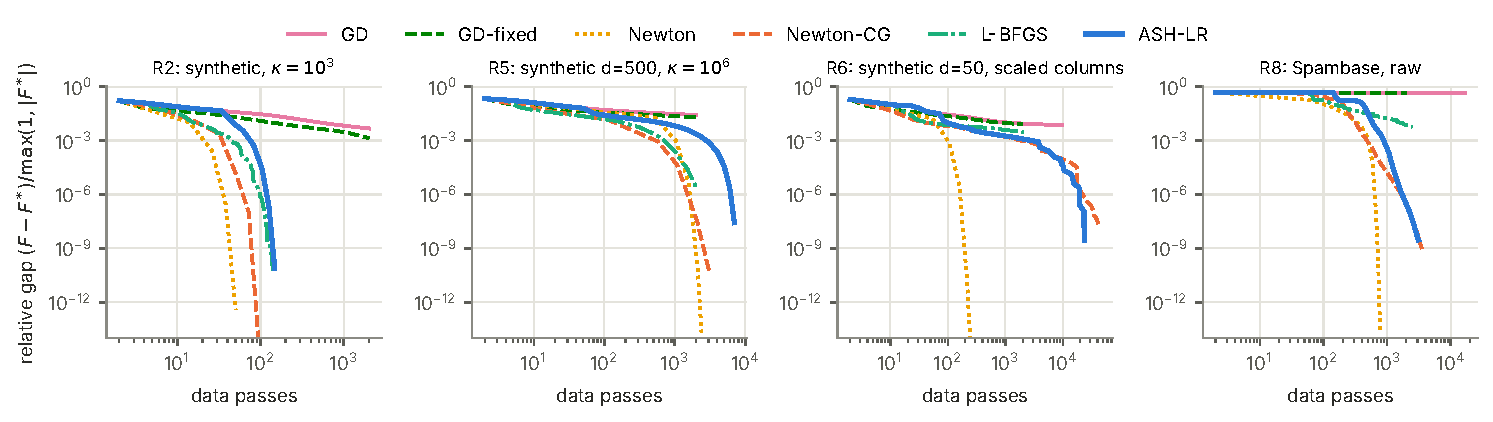
\includegraphics[width=\textwidth]{convergence_passes}
\caption{Relative objective gap versus data passes (seed 1000, log--log scale) in four
regimes. Direct Newton (dotted) reaches machine precision in a few hundred passes
in R6 and R8, where the matrix-free methods need tens of thousands.}\label{fig:conv}
\end{figure}

\subsection{Pre-registered hypothesis H1}
\Cref{tab:h1} gives, for the five primary regimes, the per-seed ratios of ASH-LR's
passes and times to those of each baseline that converged on all seeds. The best
converging matrix-free baseline was Newton--CG in all five regimes, and the change in
median passes of ASH-LR relative to it was $+111\%$ (R3), $+126\%$ (R4), $+127\%$
(R5), $+17\%$ (R6) and $+18\%$ (R8). ASH-LR therefore did not achieve the required
reduction of $20\%$ in any regime, and \textbf{H1 is not supported}. In R6 the
median per-seed ratio is $0.93$ and the Wilcoxon test does not detect a difference
($p=0.92$): ASH-LR was cheaper on some seeds and more expensive on others, and the
ratio of the medians ($1.17$) and the median of the ratios ($0.93$) point in
different directions, which itself indicates that the two methods are on a par there.

\begin{table}[t]
\centering
\caption{H1: per-seed ratios ASH-LR / baseline (median and interquartile range for
passes, median for time) and the two-sided Wilcoxon signed-rank $p$-value for passes
(ten seeds). Ratios below one favour ASH-LR. Baselines that did not converge on all
seeds are not compared.}\label{tab:h1}
\footnotesize
\begin{tabular}{llrrrr}
\toprule
Regime & Baseline & Conv. (base) & Passes ratio & Time ratio & $p$ (passes) \\
\midrule
R3 & Newton-CG & 10/10 & 2.03 [1.87, 2.56] & 2.31 & 0.002 \\
 & L-BFGS & 10/10 & 0.71 [0.54, 0.74] & 0.20 & 0.002 \\
 & Newton & 10/10 & 5.26 [4.79, 6.10] & 5.25 & 0.002 \\
\midrule
R4 & Newton-CG & 10/10 & 2.33 [1.99, 2.74] & 2.34 & 0.002 \\
 & L-BFGS & 10/10 & 1.80 [1.76, 2.08] & 1.21 & 0.002 \\
 & Newton & 10/10 & 1.65 [1.62, 1.92] & 9.51 & 0.002 \\
\midrule
R5 & Newton-CG & 10/10 & 2.25 [2.23, 2.30] & 2.26 & 0.002 \\
 & L-BFGS & 0/10 & \multicolumn{3}{c}{baseline not converged} \\
 & Newton & 10/10 & 2.68 [2.68, 2.70] & 16.92 & 0.002 \\
\midrule
R6 & Newton-CG & 10/10 & 0.93 [0.80, 1.30] & 0.85 & 0.922 \\
 & L-BFGS & 0/10 & \multicolumn{3}{c}{baseline not converged} \\
 & Newton & 10/10 & 204.40 [142.02, 238.40] & 252.76 & 0.002 \\
\midrule
R8 & Newton-CG & 10/10 & 1.17 [1.12, 1.31] & 1.28 & 0.014 \\
 & L-BFGS & 0/10 & \multicolumn{3}{c}{baseline not converged} \\
 & Newton & 10/10 & 4.15 [4.02, 4.45] & 9.02 & 0.002 \\
\bottomrule
\end{tabular}
\end{table}

\Cref{fig:ratios} extends the comparison to all regimes. ASH-LR uses between about
1.2 and 2.3 times the passes of Newton--CG, except in R6, and the ratio to direct
Newton grows to two orders of magnitude in the badly scaled synthetic regime.

\begin{figure}[t]
\centering
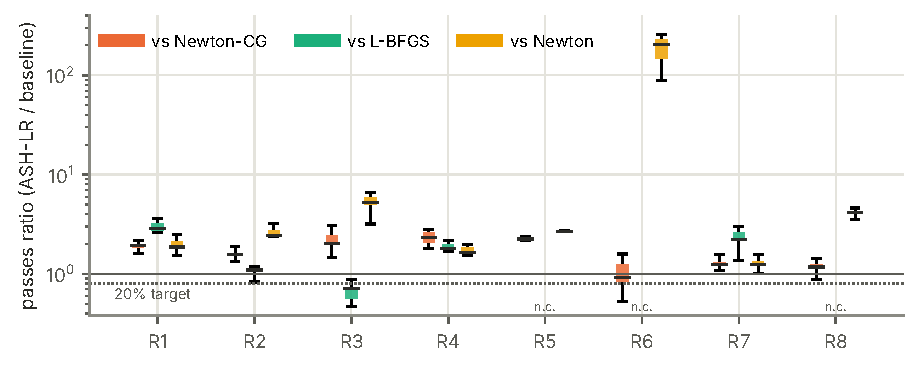
\includegraphics[width=0.85\textwidth]{ratios}
\caption{Ratio of data passes, ASH-LR over each baseline, across the ten seeds of
every regime (boxes: interquartile range; line: median). Values below the solid line
favour ASH-LR; the dotted line marks the 20\% target. ``n.c.'': baseline not converged
on all seeds.}\label{fig:ratios}
\end{figure}

\subsection{Ablation (E3)}
\Cref{tab:ablation} isolates the components of ASH-LR, and \cref{fig:ablation}
displays the median passes.

\begin{table}[t]
\centering
\caption{E3: ablation of ASH-LR (ten seeds, $w_0=0$). Conv.\ = seeds converged;
Passes = median data passes. (a) is the Milestone~2 method and (d) the final method.}\label{tab:ablation}
\footnotesize
\begin{tabular}{lrrrrrrrr}
\toprule
Variant & \multicolumn{2}{c}{R2} & \multicolumn{2}{c}{R5} & \multicolumn{2}{c}{R6} & \multicolumn{2}{c}{R8} \\
 & Conv. & Passes & Conv. & Passes & Conv. & Passes & Conv. & Passes \\
\midrule
(a) M2: direct+LS, fixed $\mu$ & 10/10 & 118 & 10/10 & 6,817 & 10/10 & 749 & 10/10 & 942 \\
(b) CG+LS, fixed $\mu$ & 10/10 & 168 & 10/10 & 6,541 & 10/10 & 48,208 & 10/10 & 2,796 \\
(c) CG+ratio, fixed $\mu$ & 10/10 & 168 & 10/10 & 6,541 & 10/10 & 48,208 & 10/10 & 3,033 \\
(d) ASH-LR (full) & 10/10 & 140 & 10/10 & 6,990 & 10/10 & 54,120 & 10/10 & 3,122 \\
(e) full, no GD phase & 10/10 & 91 & 10/10 & 5,686 & 10/10 & 39,316 & 10/10 & 3,192 \\
(f) direct+ratio, grad $\mu$ & 10/10 & 105 & 10/10 & 6,817 & 10/10 & 644 & 10/10 & 912 \\
\bottomrule
\end{tabular}
\end{table}

\begin{figure}[t]
\centering
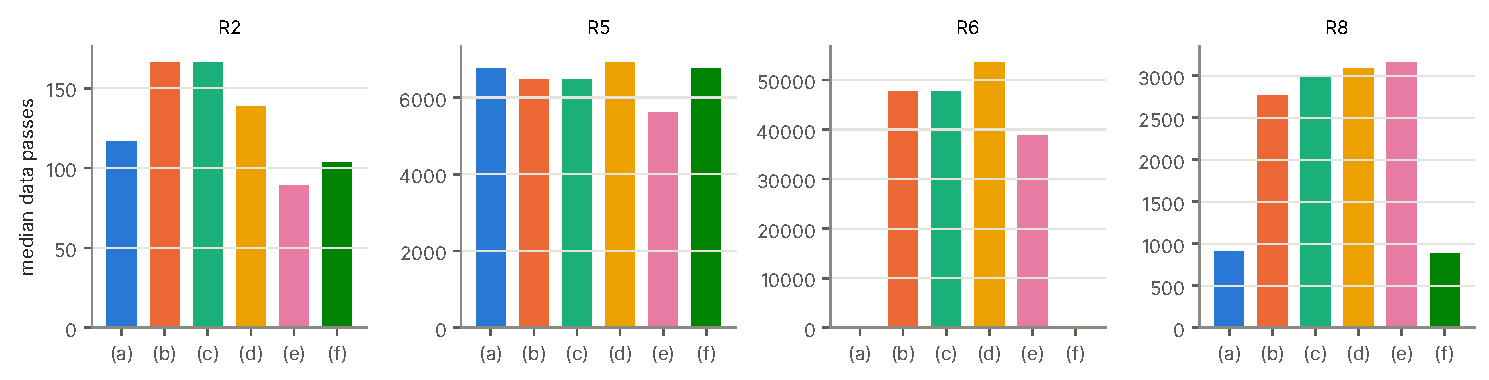
\includegraphics[width=\textwidth]{ablation}
\caption{E3: median data passes of the six ASH-LR variants.}\label{fig:ablation}
\end{figure}

\paragraph{The gradient phase is the main overhead} Removing it (variant e) reduced
the median passes in R2, R5 and R6 (by 35\%, 19\% and 27\%) and, in R2 and R5,
cut the number of iterations by roughly 70\%. Only on raw Spambase did it help slightly (3,121 vs.
3,193 passes). Because Newton's method on the logistic loss is well behaved from
$w_0=0$, as also observed for truncated Newton methods on linear
classification~\cite{galli2022truncated}, the
cautious start that motivated the gradient phase is rarely needed. This finding is
post hoc: the final method was frozen with the gradient phase, as specified.

\paragraph{The inner solver dominates in badly scaled problems} In R6 and R8 the dense-solve
variants (a) and (f) needed only 16--21 iterations, whereas every CG variant needed
434--598 iterations in R6 and 67--80 in R8. The cause is the inexact
solve: with a Hessian condition number around $10^{8}$--$10^{9}$ at the start
(\cref{tab:regimes}), unpreconditioned CG cannot reduce the residual by the forcing
factor within $d$ iterations, so the Newton steps are poor and many of them are
needed. Damping cannot repair this: in R8 the ratio test rejected a median of 18
trial steps per run, and the trace in \cref{fig:trace} shows $\mu$ jumping to about
$20$ after a series of rejections before it decays geometrically with the
gradient norm.

\paragraph{Damping rules} The gradient-regularized rule helped when combined with an
exact solve (f vs.\ a: 11\%, 14\% and 3\% fewer passes in R2, R6 and R8). With CG, it
was slightly worse than the fixed rule in R5, R6 and R8 (d vs.\ c), because a larger
$\mu$ early in the Newton phase makes the CG systems easier but the steps shorter.
Variants (b) and (c) produced identical iterates in R2, R5 and R6: when every trial
step is accepted with $\rho>0.75$, the ratio test and the line-search rule both
halve $\mu$, so the two rules only differ on problems with rejected steps.

\begin{figure}[t]
\centering
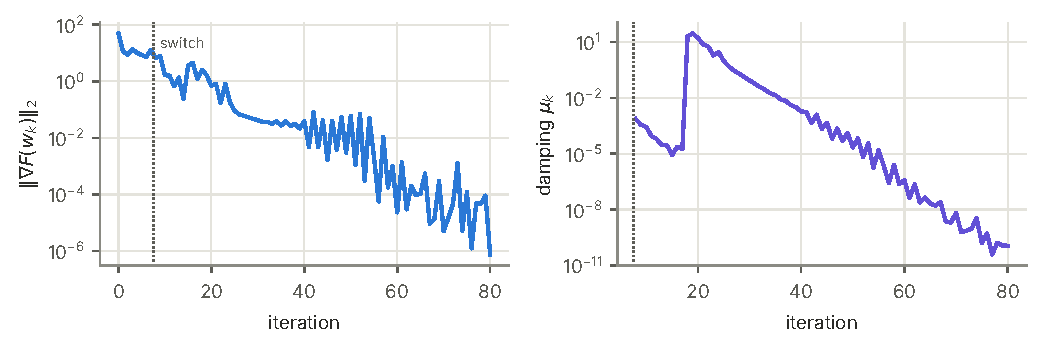
\includegraphics[width=0.85\textwidth]{trace_R8}
\caption{ASH-LR on R8 (seed 1000): gradient norm and damping per iteration. The
dotted line marks the switch to the Newton phase.}\label{fig:trace}
\end{figure}

\subsection{Robustness to starting point and regularization (E2)}
\Cref{tab:robust} summarizes 81 problems per method (three regimes, three seeds,
three values of $\lambda$, three starting points). ASH-LR, Newton and Newton--CG
converged on all 81 problems, never produced a non-finite value and never failed a
line search. L-BFGS converged on 47 of 81; it failed on 25 of the 27 raw-Spambase
problems and on all nine R5 problems with $\lambda=10^{-6}$. Robustness is thus shared by all three Newton-type
methods and is not a distinguishing advantage of ASH-LR. A distant start hurt
ASH-LR most: on R2 its median work grew from 122 passes ($w_0=0$) to 1,080 (far
start), because with saturated logits the gradient is small and the switching rule
keeps the method in the slow gradient phase for longer. Newton--CG grew only from
88 to 132 passes. Larger $\lambda$ improves the conditioning and reduced the work of
all methods; for $\lambda=10^{-2}$ Newton--CG needed a median of 86 passes against
380 for ASH-LR.

\begin{table}[t]
\centering
\caption{E2: seeds converged and, in parentheses, median data passes over the three
seeds and three values of $\lambda\in\{10^{-6},10^{-4},10^{-2}\}$ (nine problems per
cell). Relative stopping rule $\norm{g}/\max(1,\norm{g_0})\le10^{-6}$.}\label{tab:robust}
\footnotesize
\begin{tabular}{llrrrr}
\toprule
Regime & Start & Newton & Newton-CG & L-BFGS & ASH-LR \\
\midrule
R2 & zero & 9/9 (50) & 9/9 (88) & 9/9 (111) & 9/9 (122) \\
 & near & 9/9 (64) & 9/9 (90) & 9/9 (99) & 9/9 (192) \\
 & far & 9/9 (96) & 9/9 (132) & 9/9 (141) & 9/9 (1,080) \\
\midrule
R5 & zero & 9/9 (2,084) & 9/9 (518) & 6/9 (426) & 9/9 (802) \\
 & near & 9/9 (3,127) & 9/9 (532) & 6/9 (470) & 9/9 (1,050) \\
 & far & 9/9 (3,662) & 9/9 (686) & 6/9 (530) & 9/9 (1,990) \\
\midrule
R8 & zero & 9/9 (595) & 9/9 (456) & 0/9 (2,508) & 9/9 (1,040) \\
 & near & 9/9 (657) & 9/9 (584) & 1/9 (2,469) & 9/9 (866) \\
 & far & 9/9 (921) & 9/9 (471) & 1/9 (2,449) & 9/9 (805) \\
\bottomrule
\end{tabular}
\end{table}

\subsection{Single precision (E4) and numerical stability (E5)}
In single precision with tolerance $10^{-4}$ (\cref{tab:f32}), all three methods
converged on R2 and standardized Spambase (R7), with objective gaps comparable to
double precision and wall times 4--55\% lower. On raw Spambase (R8), however,
Newton--CG converged on none and ASH-LR on one of three seeds, while direct Newton
converged on all. With a Hessian condition number near $10^{9}$, which exceeds
$1/\epsilon_{\text{float32}}\approx1.7\times10^{7}$, the rounding errors in the
Hessian-vector products and CG recurrences~\cite{higham2022mixed} are large enough to make the inexact
Newton steps unreliable, whereas the dense factorization still delivers usable
steps. Single precision is therefore safe only for reasonably scaled data when the
inner solver is CG.

\begin{table}[t]
\centering
\caption{E4: float64 versus float32 (tolerance $10^{-4}$, three seeds). Median
relative gap of the returned solution evaluated in float64, and ratio of median wall
times.}\label{tab:f32}
\footnotesize
\begin{tabular}{llrrrrr}
\toprule
Regime & Method & \multicolumn{2}{c}{Conv.} & \multicolumn{2}{c}{Median gap} & Time ratio \\
 & & f64 & f32 & f64 & f32 & f32/f64 \\
\midrule
R2 & Newton & 3/3 & 3/3 & 2.1e-13 & 2.4e-13 & 0.79 \\
 & Newton-CG & 3/3 & 3/3 & 1.2e-08 & 1.1e-06 & 0.93 \\
 & ASH-LR & 3/3 & 3/3 & 7.8e-07 & 8.9e-07 & 0.96 \\
\midrule
R7 & Newton & 3/3 & 3/3 & 2.7e-09 & 2.8e-09 & 0.57 \\
 & Newton-CG & 3/3 & 3/3 & 1.9e-07 & 2.4e-07 & 0.45 \\
 & ASH-LR & 3/3 & 3/3 & 1.1e-05 & 3.2e-07 & 0.53 \\
\midrule
R8 & Newton & 3/3 & 3/3 & 1.0e-10 & 1.0e-10 & 0.58 \\
 & Newton-CG & 3/3 & 0/3 & 1.8e-05 & 5.9e-05 & 29.38 \\
 & ASH-LR & 3/3 & 1/3 & 3.3e-05 & 3.0e-05 & 37.60 \\
\bottomrule
\end{tabular}
\end{table}

\Cref{tab:stab} reports the stability test from an extreme starting point (logit
standard deviation $10^3$). With the stable formulas both methods converged on every
problem in double precision. With the naive formulas the initial loss overflows to
$+\infty$; every subsequent trial point whose margins still exceed the overflow
threshold also evaluates to $+\infty$, so line searches and ratio tests cannot
compare candidates. ASH-LR failed in all twelve naive runs, and Newton recovered in
only three of the six double-precision runs, when its first full step happened to
land at finite values. In single precision, where $\exp$ overflows already beyond
$|z|\approx88$, all naive runs failed. The only failures with the stable formulas
were the ASH-LR runs on R8 in float32, which reached the iteration limit with finite
values, consistent with the CG precision issue above. Stable evaluation is cheap and
exact, and it is the one component of ASH-LR whose benefit is unconditional.

\begin{table}[t]
\centering
\caption{E5: seeds converged out of three from an extreme start (logit standard
deviation $10^3$) with stable and naive formulas.}\label{tab:stab}
\footnotesize
\begin{tabular}{lllrrl}
\toprule
Regime & Precision & Formulas & Newton & ASH-LR & Failure mode \\
\midrule
R2 & float64 & stable & 3/3 & 3/3 & -- \\
 & float64 & naive & 2/3 & 0/3 & non finite \\
 & float32 & stable & 3/3 & 3/3 & -- \\
 & float32 & naive & 0/3 & 0/3 & non finite \\
\midrule
R8 & float64 & stable & 3/3 & 3/3 & -- \\
 & float64 & naive & 1/3 & 0/3 & non finite \\
 & float32 & stable & 3/3 & 0/3 & max iter \\
 & float32 & naive & 0/3 & 0/3 & non finite \\
\bottomrule
\end{tabular}
\end{table}

\subsection{Discussion}
The results give a consistent picture of when the ideas behind ASH-LR pay off.

\emph{Stable evaluation} is necessary, not optional: it costs nothing, changes no
iterate when the naive formulas are finite, and prevents total failure from distant
starting points or in single precision.

\emph{Second-order information} is what makes ill-conditioned logistic regression
tractable: all Newton-type methods converged everywhere, while first-order methods
and, on badly scaled data, L-BFGS did not. This supports the premise of the project.

\emph{The hybrid structure} did not pay off in our regimes. The gradient phase costs
15--40 passes that Newton-type methods do not need from $w_0=0$, and it becomes
expensive from distant starts. The damping mechanism worked as designed---$\mu$
grew after rejected steps and vanished near the solution---but with CG as the inner
solver the bottleneck in badly scaled problems is the accuracy of the inner solve,
which damping cannot fix. A diagonal (Jacobi) or randomized Nystr\"om
preconditioner~\cite{frangella2023randomized}, or simply feature scaling, would
attack the actual cause; the dramatic difference between R7 and R8, which differ
only by standardization, makes the same point from the data side.

\emph{Passes versus time.} For $d\le500$ dense features, the BLAS-3 Hessian
formation of direct Newton runs so much faster per flop than the matrix--vector
products of CG that direct Newton wins in time even where it loses in passes (R4).
Matrix-free methods become necessary only when $d$ is so large that $d^2$ memory or
$d^3$ work is prohibitive, or when $X$ is sparse; our experiments do not cover that
regime, so they cannot show whether ASH-LR would then compete with Newton--CG.

\paragraph{Threats to validity} Timings come from one virtual machine with two cores
and three repetitions; passes, which are machine-independent, lead to the same
conclusions. The synthetic designs have log-spaced spectra and logistic labels and
may be easier or harder than real data. Spambase contains 391 duplicate rows, which
affects test accuracy but not the optimization comparison. Finally, the ASH-LR
parameters (switching thresholds, $\mu_0$, update factors) were not tuned. The
ablation bounds what tuning the switch could achieve: even with no gradient phase at
all (variant e), ASH-LR matched Newton--CG in R2 (91 vs.\ 92 passes), used 15\%
fewer passes in R6 (39,316 vs.\ 46,162), and stayed behind in R5 and R8. This
post-hoc observation suggests that a damped Newton--CG without the gradient phase may
be competitive on badly scaled problems, but it would need its own pre-registered
test.


\section{Conclusions}\label{sec:conclusion}

We implemented and evaluated ASH-LR, a hybrid method for ill-conditioned
$\ell_2$-regularized logistic regression that combines stable loss evaluation, an
initial gradient phase, and a damped inexact Newton--CG phase with a ratio test and
gradient-regularized damping $\mu_k=\sqrt{\theta_k\norm{g_k}}$. The evaluation
followed a plan fixed before the final experiments, with eight regimes, ten seeds,
five baselines and four supplementary experiments.

ASH-LR converged on every problem in double precision, including those where
gradient descent and L-BFGS failed, and stable evaluation was essential for
convergence from distant starting points. However, the pre-registered efficiency
hypothesis was not supported: in none of the five primary ill-conditioned regimes
did ASH-LR reduce the work of the best matrix-free baseline, Newton--CG, by 20\%;
it required 18\% to 127\% more data passes in four regimes and was statistically on
a par in one badly scaled regime. Direct Newton was the fastest method throughout the dimensions
studied ($d\le500$). The ablation located the causes: the gradient phase adds work
that Newton-type methods do not need from $w_0=0$, and in badly scaled problems the
accuracy of the unpreconditioned CG solve, not the damping, limits progress.

For practitioners, the results suggest a simple rule: evaluate the loss stably, use
direct Newton when $d$ is small enough to form the Hessian, and otherwise use
Newton--CG, preferably on standardized features. Future work should
(i) add a diagonal or randomized Nystr\"om preconditioner~\cite{frangella2023randomized} to the CG solver, which targets the observed
bottleneck; (ii) test damped Newton--CG without the gradient phase, which the
ablation identified as promising on badly scaled data, in a new pre-registered study;
(iii) extend the evaluation to high-dimensional sparse data, where matrix-free
methods are the only option; and (iv) analyse the convergence of the
gradient-regularized ratio-test rule with inexact solves.

\section*{Code and data availability}
The implementation, tests, experiment scripts, raw results and the pre-registered
plan are available in the project repository (see the README for the URL). Spambase is
available from the UCI Machine Learning Repository under CC BY 4.0~\cite{spambase}.


\bibliographystyle{elsarticle-num}
\bibliography{references}

\end{document}
